\documentclass{article}
\usepackage[utf8]{inputenc}
\usepackage{float}
\usepackage{xcolor}
\usepackage{graphicx}

\usepackage{hyperref}
\hypersetup{
    colorlinks=true,
    linkcolor=blue,
    filecolor=magenta,      
    urlcolor=blue,
}

\title{Scientific Computing - Molecular dynamics \\ Group F}
\newcommand{\subtitle}{Problem sheet 1}
\author{
    Jimin Kim \\
    Christian Nix \\
    Noah Schlenker
}
\date{\today}

\begin{document}

\maketitle

\begin{center}
    \LARGE \subtitle{}
\end{center}

\section{Pull request}
The pull request can be found \href{https://github.com/noahpy/MolSim-SS24/pull/10}{here}.

\section{First Steps}

\begin{itemize}
    \item Nothing interesting to report, as everything went well and we could install without any problems
    \item Only thing worthwhile mentioning is how we setup the system for Mac (may be interesting to other groups)
    \begin{itemize}
        \item Create a docker image with all required libraries installed
        \item Integrate it into a Clion tool chain
        \item Configure Clions build to use the docker image
        \item This is essentially the same as described on the problem sheet for Windows and WSL 
    \end{itemize}
\end{itemize}

\section{First Pull Request}

\begin{itemize}
    \item We created a basic README with all required information as per the work sheet
    \item The build instructions were mainly taken from the submission guidelines
    \item We then created the pull request using Github's interface
    \item We later expanded the README to be more detailed
    \item A link to the pull request can be found \href{https://github.com/noahpy/MolSim-SS24/pull/1}{here}
    \item \emph{Please note that we are aware that the documentation cannot be built on the branch that we created the initial pull request for, as the documentation was only added later with another branch}
\end{itemize}

\section{Completion of the program frame}

\subsection{Naive Velocity-Störmer-Verlet}
\begin{itemize}
    \item We naively implemented the formulas described in the slides
    \begin{itemize}
        \item Positions: $x_i(t_{n+1}) = x_i(t_{n}) + \Delta t \cdot v_i(t_n) + (\Delta t )^2 \frac{F_i(t_n)}{2m_i}$
        \item Velocities: $v_i(t_{n+1}) = v_i(t_n) + \Delta t \frac{F_i(t_n) + F_i(t_{n+1})}{2m_i}$
        \item Forces: $F_i = \sum_{j=1, j \neq i}^{\#particles}
        \frac{m_im_j}{(||x_i-x_j||_2)^3} (x_j - x_i) $
        \item For this we utilized the array helper functions given to us within the \verb|utils| folder
    \end{itemize}
    \item The VTK-output was basically a simple drop in replacement which did not make any problems
    \begin{itemize}
        \item During the refactoring described later in \ref{sec:Refactoring}, we needed to slightly adapted the VTK Output writer to take the simulation object as a parameter
        \item We did not manage to generate binary outputs, even though the benefit of having smaller output files is tempting
        \item This may become relevant, as soon as the simulation is run for longer periods of time i.e. more files are written
        \item We also question the necessaty to write a file for every iteration. We intend to tackle this in the next assignment
    \end{itemize}
    \item We implemented command line arguments using \verb|getopt|
    \begin{itemize}
        \item This is the typical c approach and we may switch to \verb|boost::program_options| in the future
        \item For now this approach seems sufficient, we adapt if needed
    \end{itemize}
\end{itemize}

\section{Simulation of Halley's Comet}

\begin{itemize}
    \item We ran the simulation as per the required arguments. You can find the video alongside our submission (step size 40 in Paraview to speed it up)
    \item The animation looks good and returns sensible results
    \item To figure out which sphere represents which celestial body, we can refer to \href{https://nssdc.gsfc.nasa.gov/planetary/factsheet/}{Nasa's fact sheet}
    \begin{itemize}
        \item Firstly, we can assume the stable sphere in the middle to be the sun, as everything orbits it
        \item Secondly, we can assume the closer sphere to be earth, as the comet is passing by closely
        \item Taking the distance of earth from the sun to be $149.6 \cdot 10^6 km$ and its distance form the earth in the input file $1$
        \item Distance unknown planet in file $= 5.36$ $\Rightarrow$ $149.6 \cdot 10^6 km \; \cdot \; 5.36 \; = 801.856 \cdot 10^6 km$ distance from sun in reality
        \item Matching this back to Nasa's sheet we get the unknown planet to be most likely Jupiter ($778.5 \cdot 10^6 km$ in reference)
    \end{itemize}    
\end{itemize}

\section{Refactoring and documentation}
\label{sec:Refactoring}

Finally to the interesting part.

\subsection{ParticleContainer}
\label{sec:Refactoring:ParticleContainer}
\begin{itemize}
    \item The \verb|ParticleContainer| class is our implementation of a data structure managing all particles of the simulation (see folder src/models)
    \item Particles are stored in a \verb|std::vector<Particle>|. This is advantageous over using \verb|std::list|, as we do not expect the number of particles to change: fast extensiblity of the container is not necessary. Additionally, we expect to loop over the particles often. Storing \verb|Particle|s in contiguous memory allows faster access, which is guaranteed when using \verb|std::vector<Particle>|.
    \item To facilitate a looping access over the particles, we implemented the \verb|begin()| and the \verb|end()| functions of our custom Container
    \item To calculate the force between particles, one needs to loop over all distinct pairs of particles. To facilitate / optimize this, we implemented an internal class \verb|PairIterator| within the \verb|ParticleContainer|, which acts as an iterator over those pairs. One can simply reach the next distinct pair by incrementing the iterator. This also avoids duplicate / twin pairs when compared to using two for-loops. See this in action in src/physics/forceCal/forceCal.cpp.
\end{itemize}

\subsection{Extensibilty of our project}
\begin{itemize}
    \item To allow for high flexibility regarding the approach of calculating the forces, velocities, and positions, we opted to implement the strategy pattern
    \item In src/physics one can find the class \verb|PhysicsStrategy| which has the different methods for calculating the physics as members i.e. \verb|calX|, \verb|calV|, and \verb|calF|
    \item When initializing \verb|PhysicsStrategy| you can pass the desired strategy of doing the physics in the simulation as parameters in the constructor. This way, the \verb|PhysicsStragey| class acts as an interface to different strategy functions, allowing to interchange different implementation quickly and observe their differences.
    \item Now, as different approaches may use different model variables, we need to find a way to standardize the function signatures. This is solved by introducing the \verb|Simulation| class, which represents the simulation flow and all its variables as a whole. The simulation class runs (\verb|Simulation::runSim()|) the simulation by using the I/O classes, model variables and \verb|PhysicsStrategy| passed to it. When doing so, it passes itself to the strategy functions, so that they have the complete access on all model variables. This allows a standardized signature over all different strategy functions, whilst assuring their access on necessary variables.
    \item Moreover, we may want to introduce new kinds of simulations with different flow of calculation / additional model variables (such as temperature, constant gravitational force). Thus, the \verb|Simulation| class is abstract and different simulation instances (child classes) can extend on this base simulation. This way, those child classes are always "backwards compatible" to parent classes, meaning they can be passed to strategy function which only require "older" simulations. This allows us to run child simulations with "older" strategy functions, which facilitates the implementation of those.
        This class is an abstract class to use as a basis for different simulations
    \item For the simulation of this problem sheet, we implemented the \verb|PlanetSimulation| class

    \item To ensure the extensiblity of the different I/O methods, we opted to use the Template method pattern,  defines the skeleton of an algorithm in the superclass but lets subclasses override specific steps of the algorithm without changing its structure.
    \item In this instance, the \verb|FileReader| and \verb|FileWriter| classes are the super classes defining the skeleton of subclasses implementing future methods. 
    \item All I/O related classes were implemented in src/io

    \item A UML-like diagram of the idea can be seen in Figure \ref{fig:strat}
    \begin{figure}[H]
        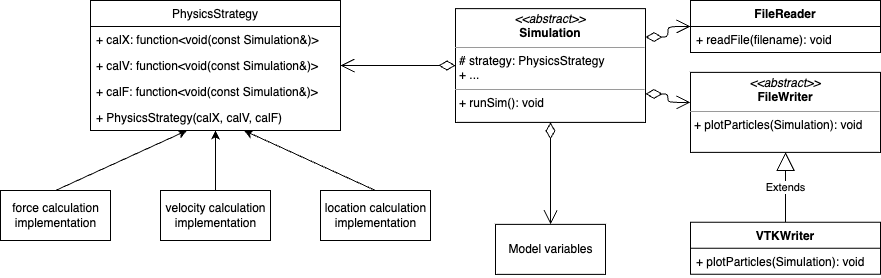
\includegraphics[width=\textwidth]{/home/jimin/MolSim2/docs/res/strategy_long}
        \caption{UML-like diagram showing our idea behind the strategy pattern}
        \label{fig:strat}
    \end{figure}

\end{itemize}

\subsection{Improving the force calculations}
\label{sec:Refactoring:forceimprovements}

\begin{itemize}
    \item We implemented a second strategy for calculating the forces in our simulation, optimizing the runtime.
    \item For this we use the simple identity $F_{i,j} = -F_{j,i}$
        \begin{equation}
            F_{i,j} = \frac{m_im_j}{(||x_i-x_j||_2)^3} (x_j - x_i) = \frac{m_jm_i}{(||x_j-x_i||_2)^3} \left(-1 \cdot \left(x_i - x_j\right)\right) = - F_{j,i} 
        \end{equation}
        Thus, one only needs to iterate over all distinct pairs (without identical pairs) of particles instead of all tuples to calculate all forces.
    \item This is implemented using the pairwise iterator mentioned in \ref{sec:Refactoring:ParticleContainer}
    \item Theoretically, this should yield a speedup of 2, as only half the number of calculations are necessary
    \item The values we measured can be seen in Table \ref{tab:speedup}. This is only a speedup of around 1.25
        \begin{table}[H]
            \centering
            \begin{tabular}{|l|l|l|l|l|}
            \hline
                & Time for $10^6$ iterations \\ \hline
            Naive & 31109ms                  \\ \hline
            V2    & 24881ms                  \\ \hline
            \end{tabular}
            \caption{Values measured for the two different force calculation strategies. One being the naive implementation, while the other utilizes $F_{1,2} = - F_{2,1}$. This yields a speedup of approx 1.25.}
            \label{tab:speedup}
        \end{table}
    \item To reproduce the numbers, simply run the test code for timing both approaches. It will load the \verb|sonne-eingabe.txt| file and run a force calculation for $10^6$ times
    \item Note that this will vary
\end{itemize}

\subsection{Testing}

\begin{itemize}
    \item Even though tests were not mandatory, we opted to integrate some basic test to check our implementation
    \item This was done using the \verb|gtest| testing library
    \item This is mainly focused on the \verb|ParticleContainer| class and its iterators
    \item But we also included a test for the two different approaches on calculating the forces as mentioned in \ref{sec:Refactoring:forceimprovements} and measuring the speedup
    \item To run the tests follow the README
\end{itemize}

\end{document}
